% Figure 2: the 1-stage H-Net we trained (configs/hnet_small.json:
% arch_layout ["m4", ["T12"], "m4"]). Bytes go up the left side, are cut into
% chunks, pass through the main Transformer once per chunk, and come back down
% the right side to predict the next byte.
\documentclass[tikz,border=10pt]{standalone}
\usepackage[T1]{fontenc}
\usepackage[scaled=0.92]{helvet}
\renewcommand{\familydefault}{\sfdefault}
\usetikzlibrary{arrows.meta,backgrounds,calc}

\definecolor{ink}{HTML}{1F1F1E}
\definecolor{quiet}{HTML}{6B6A66}
\definecolor{accent}{HTML}{2A78D6}
\definecolor{accentsoft}{HTML}{E4EEFB}
\definecolor{greysoft}{HTML}{EFEEEA}
\definecolor{greyline}{HTML}{A8A69E}
\definecolor{band}{HTML}{F7F6F2}

\newcommand{\vsp}{\textcolor{quiet}{\textbullet}}
\newcommand{\cw}{0.42}

% \bytestrip{x of centre}{y}{characters}{cells to highlight (1-based)}
\newcommand{\bytestrip}[4]{%
  \foreach \c [count=\i from 0] in {#3} {%
    \draw[greyline, fill=white, line width=0.5pt]
      ({#1+(\i-5)*\cw}, {#2-0.21}) rectangle ({#1+(\i-4)*\cw}, {#2+0.21});
  }%
  \foreach \h in {#4} {%
    \draw[accent, fill=accentsoft, line width=0.7pt]
      ({#1+(\h-6)*\cw}, {#2-0.21}) rectangle ({#1+(\h-5)*\cw}, {#2+0.21});
  }%
  \foreach \c [count=\i from 0] in {#3} {%
    \node[text=ink, font=\ttfamily\footnotesize, inner sep=0pt] at ({#1+(\i-4.5)*\cw}, {#2}) {\strut\c};
  }%
}

% \chunkstrip{x of centre}{y}: four chunk vectors
\newcommand{\chunkstrip}[2]{%
  \foreach \i in {0,1,2,3} {%
    \draw[accent, fill=accentsoft, line width=0.7pt, rounded corners=1.5pt]
      ({#1+(\i-2)*0.5+0.04}, {#2-0.23}) rectangle ({#1+(\i-1)*0.5-0.04}, {#2+0.23});
  }%
}

\begin{document}
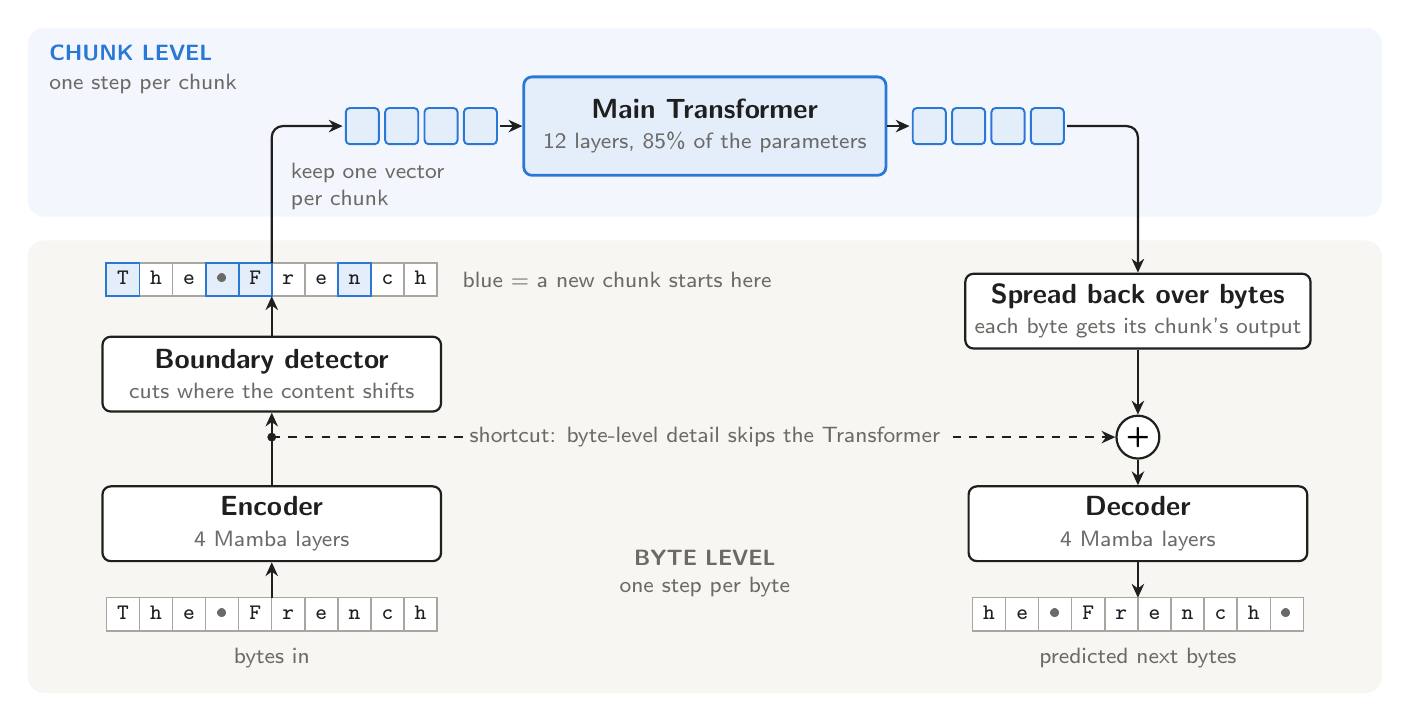
\begin{tikzpicture}[
    >={Stealth[length=5pt,width=4.5pt]},
    flow/.style={->, line width=0.8pt, draw=ink},
    block/.style={draw=ink, fill=white, line width=0.8pt, rounded corners=3pt,
                  minimum width=4.3cm, minimum height=0.95cm, align=center, text=ink},
    main/.style={block, draw=accent, fill=accentsoft, line width=1pt,
                 minimum width=4.6cm, minimum height=1.25cm},
    small/.style={font=\footnotesize, text=quiet},
    note/.style={font=\footnotesize, text=quiet, align=left},
  ]

  % background bands: byte level below, chunk level above
  \begin{scope}[on background layer]
    \fill[band, rounded corners=6pt] (-3.1,-1.0) rectangle (14.1,4.75);
    \fill[accentsoft!45, rounded corners=6pt] (-3.1,5.05) rectangle (14.1,7.45);
  \end{scope}
  \node[font=\footnotesize\bfseries, text=quiet] at (5.5,0.72) {BYTE LEVEL};
  \node[small] at (5.5,0.35) {one step per byte};
  \node[anchor=north west, font=\footnotesize\bfseries, text=accent] at (-2.95,7.35) {CHUNK LEVEL};
  \node[anchor=north west, small] at (-2.95,6.98) {one step per chunk};

  % ---------------- left column: bytes in, going up
  \bytestrip{0}{0}{T,h,e,\vsp,F,r,e,n,c,h}{}
  \node[small] at (0,-0.55) {bytes in};

  \node[block] (enc) at (0,1.15) {\textbf{Encoder}\\[-1pt]{\footnotesize\color{quiet}4 Mamba layers}};
  \node[block] (det) at (0,3.05) {\textbf{Boundary detector}\\[-1pt]{\footnotesize\color{quiet}cuts where the content shifts}};

  \bytestrip{0}{4.25}{T,h,e,\vsp,F,r,e,n,c,h}{1,4,5,8}
  \node[note, anchor=west] at (2.3,4.25) {blue = a new chunk starts here};

  \draw[flow] (0,0.21) -- (enc.south);
  \draw[flow] (enc.north) -- (det.south);
  \draw[flow] (det.north) -- (0,4.04);

  % ---------------- top: one vector per chunk through the main Transformer
  \chunkstrip{1.9}{6.2}
  \node[main] (tr) at (5.5,6.2) {\textbf{Main Transformer}\\[-1pt]{\footnotesize\color{quiet}12 layers, 85\% of the parameters}};
  \chunkstrip{9.1}{6.2}

  \draw[flow, rounded corners=4pt] (0,4.46) -- (0,6.2) -- (0.9,6.2);
  \node[note, anchor=north west] at (0.12,5.85) {keep one vector\\per chunk};
  \draw[flow] (2.9,6.2) -- (tr.west);
  \draw[flow] (tr.east) -- (8.1,6.2);

  % ---------------- right column: back to bytes, going down
  \node[block] (dechunk) at (11,3.85) {\textbf{Spread back over bytes}\\[-1pt]{\footnotesize\color{quiet}each byte gets its chunk's output}};
  \node[draw=ink, fill=white, circle, line width=0.8pt, inner sep=1.5pt, font=\bfseries] (plus) at (11,2.25) {+};
  \node[block] (dec) at (11,1.15) {\textbf{Decoder}\\[-1pt]{\footnotesize\color{quiet}4 Mamba layers}};
  \bytestrip{11}{0}{h,e,\vsp,F,r,e,n,c,h,\vsp}{}
  \node[small] at (11,-0.55) {predicted next bytes};

  \draw[flow, rounded corners=4pt] (10.1,6.2) -- (11,6.2) -- (dechunk.north);
  \draw[flow] (dechunk.south) -- (plus.north);
  \draw[flow] (plus.south) -- (dec.north);
  \draw[flow] (dec.south) -- (11,0.21);

  % ---------------- shortcut around the Transformer
  \fill[ink] (0,2.25) circle (1.6pt);
  \draw[flow, dashed] (0,2.25) -- (plus.west);
  \node[note, fill=band, inner sep=2pt] at (5.5,2.25) {shortcut: byte-level detail skips the Transformer};
\end{tikzpicture}
\end{document}
